\section{Design}
\subsection{Generator}
The generator resides in the \texttt{de.hs\_rm.cs.vs.dsm.flow} plug-in project 
in the package \texttt{de.hs\-\_rm.\-cs.vs.dsm.flow.generator} and consists of 
two parts. The first part is a script written in the Xtend \cite{xtend} language 
which controls the transformation process of the query language to the target 
platform. It is the main entry point for the customization of the code 
generation process of the query language. The Xtend intepreter generates 
Java interfaces and classes which are stored in the \texttt{src-gen/} directory
in the same project and package. The second part of the generator are a set of
classes which are used for the target platform representation of code written in
the query language. Figure \ref{fig:generator} depicts the corresponding classes
and their relation. The figure omits method and attribute details which are 
described later in that section.
\begin{figure}[htpb]
  \centering
  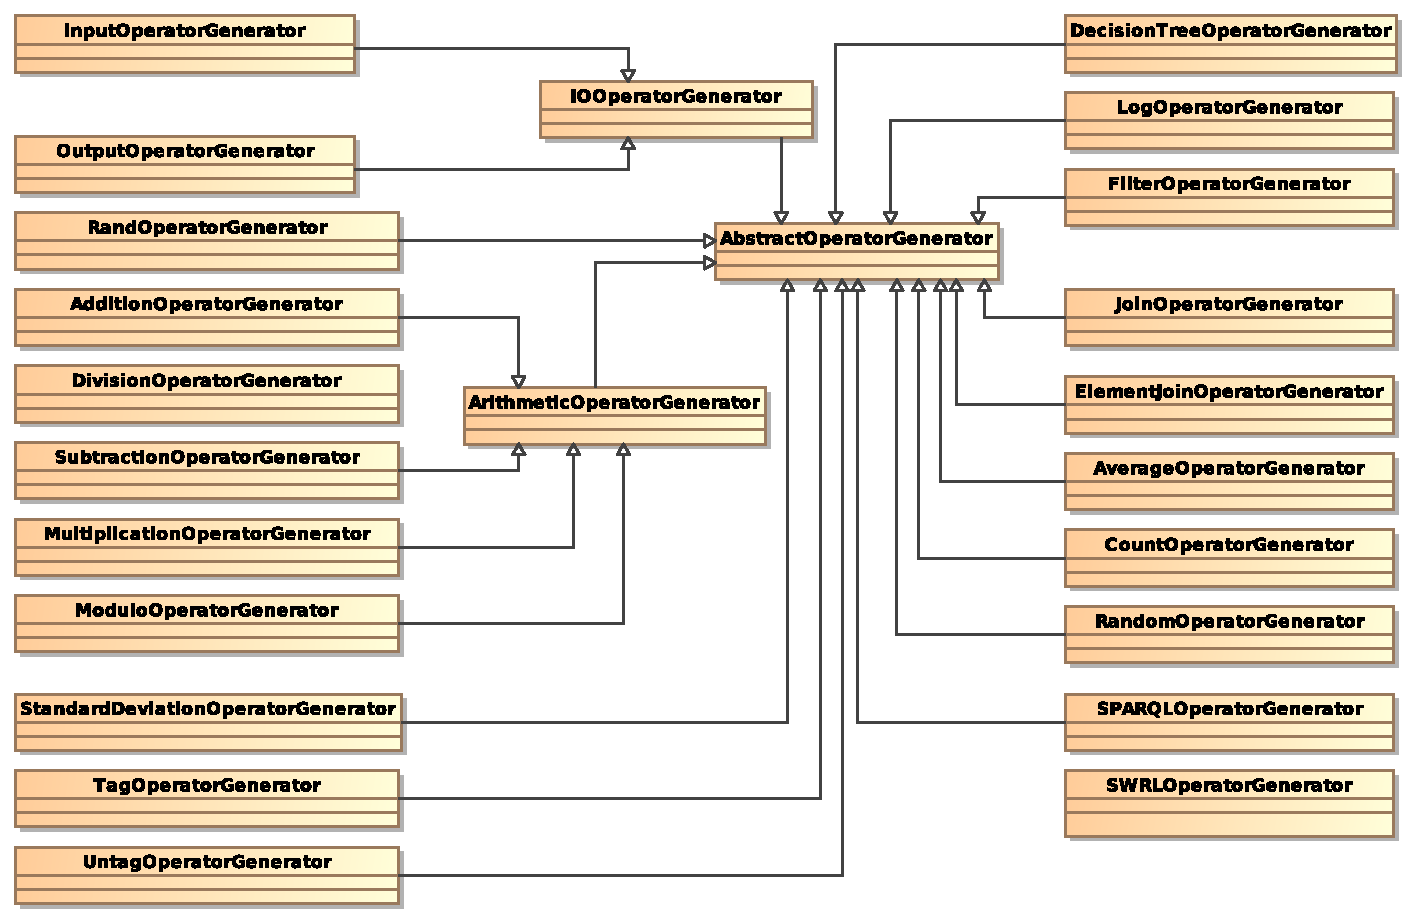
\includegraphics[width=0.8\textwidth]{figures/overview}
  \caption{\emph{Overview of classes which are used in code generation}}
  \label{fig:generator}
\end{figure}
\subsubsection{Bla}

